

\begin{figure}[H]
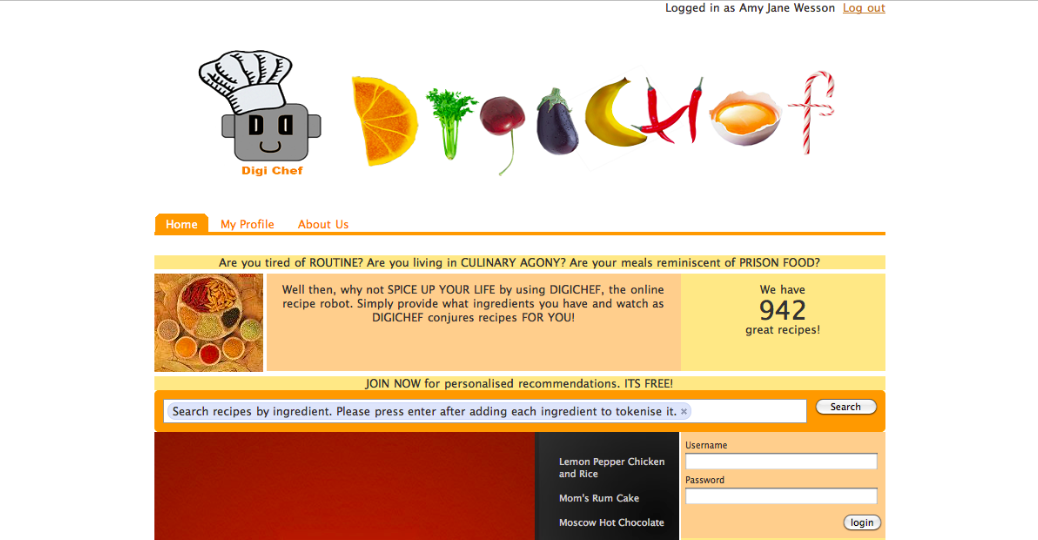
\includegraphics[width=1\textwidth]{result_index}[H]
\caption{Homepage}
\label{fig:result_index}
\end{figure}

Orange colour is features prominently in our website design, given the fact that it is an appetite stimulating colour. In addition, an attractive banner, which is decorated with fruits and vegetables was designed. The banner also features the digichef mascot, which provides us with a tool with which we can better market our website.
The search box on the index page not only allows users to input ingredients to search for recipes, but also provides an auto-completion functionality which provides affirmation as a user types an ingredient. There is also a sign-in box which allows users access to a profile.

\begin{figure}[H]
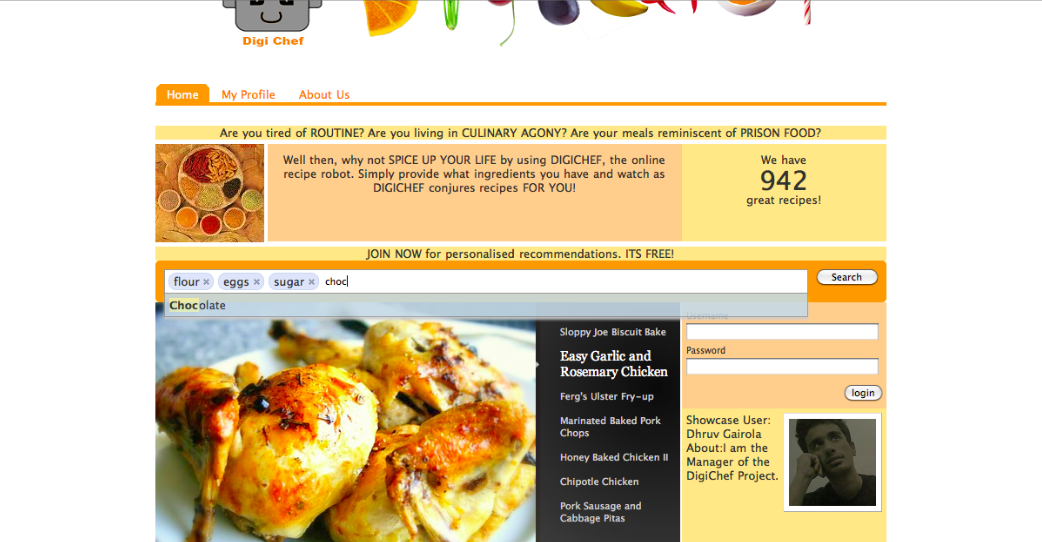
\includegraphics[width=1\textwidth]{result_index2}[H]
\caption{Homepage}
\label{fig:result_index2}
\end{figure}

Fig~\ref{fig:result_index2} denotes the results of the JavaScripts slideshow, the auto complete search box, and the user of the week. Notice the recipe name on the right hand side of the slideshow, clicking these generates the image of that recipe in the left part of the slideshow. Clicking on the image itself, causes the page to redirect to the recipe itself. Refreshing the page each time loads a new slideshow with completely new recipes.

\begin{figure}[H]
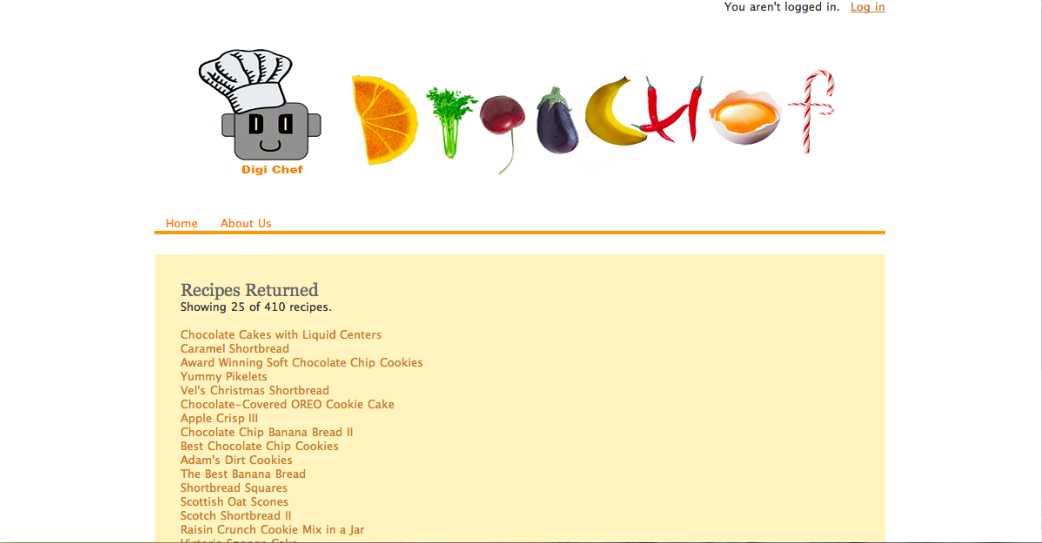
\includegraphics[width=1\textwidth]{result_list}[H]
\caption{Search Result}
\label{fig:result_list}
\end{figure}

Fig~\ref{fig:result_list} shows a recipe list which was generated based on the ingredients entered by the users.

\begin{figure}[H]
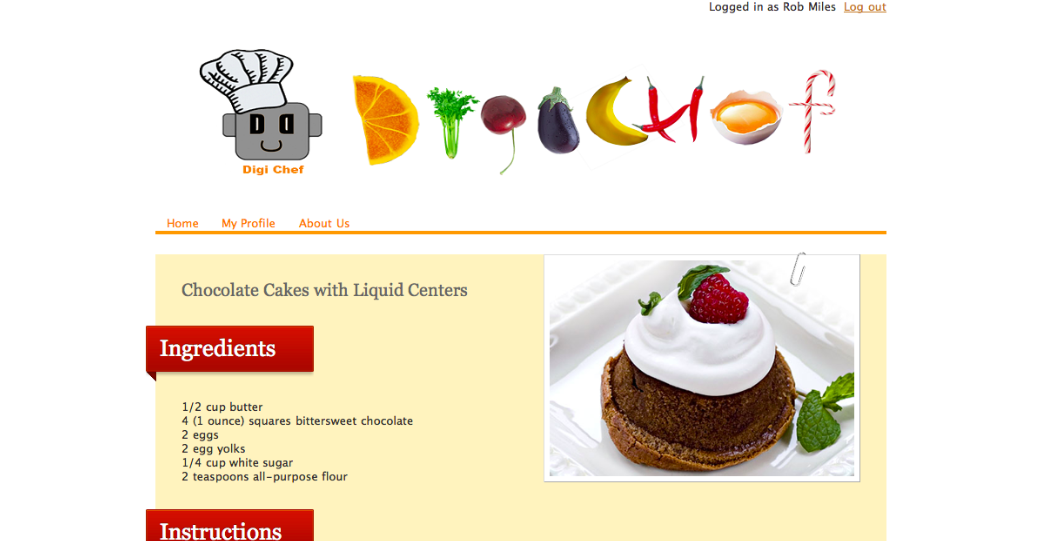
\includegraphics[width=1\textwidth]{result_recipe}
\caption{Recipe Page}
\label{fig:result_recipe}
\end{figure}

\begin{figure}[H]
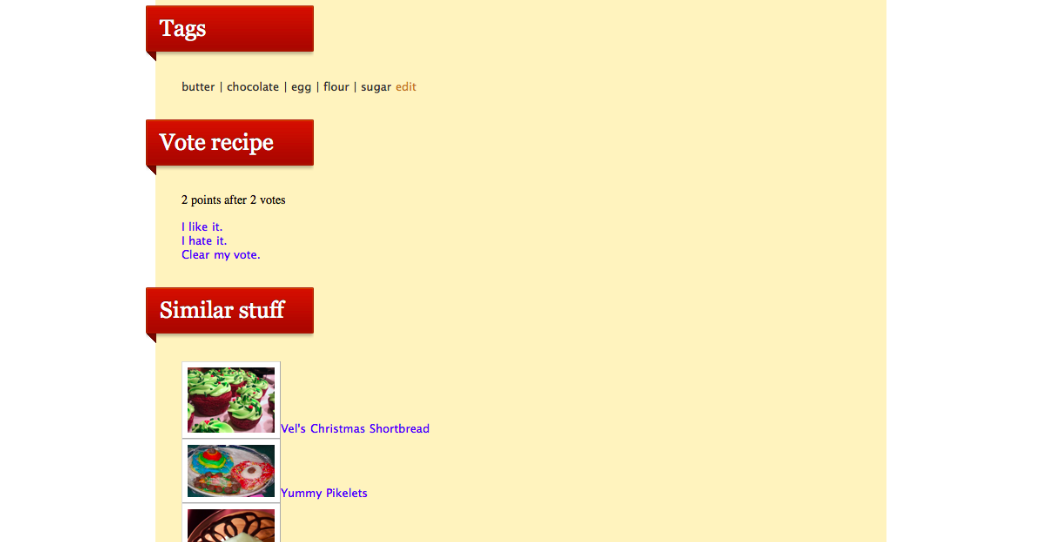
\includegraphics[width=1\textwidth]{result_recipe2}[H]
\caption{Recipe Page}
\label{fig:result_recipe2}
\end{figure}

Fig~\ref{fig:result_recipe} and Fig~\ref{fig:result_recipe2} shows what the version 2 recipe page looks like. It features the basic information about the recipe, along with an image of the recipe, and also allows users to vote on a recipe, provided they are logged in. Moreover, users with profiles will also get personalised recommendations of recipes based on the recipe liked by similar users.

\begin{figure}[H]
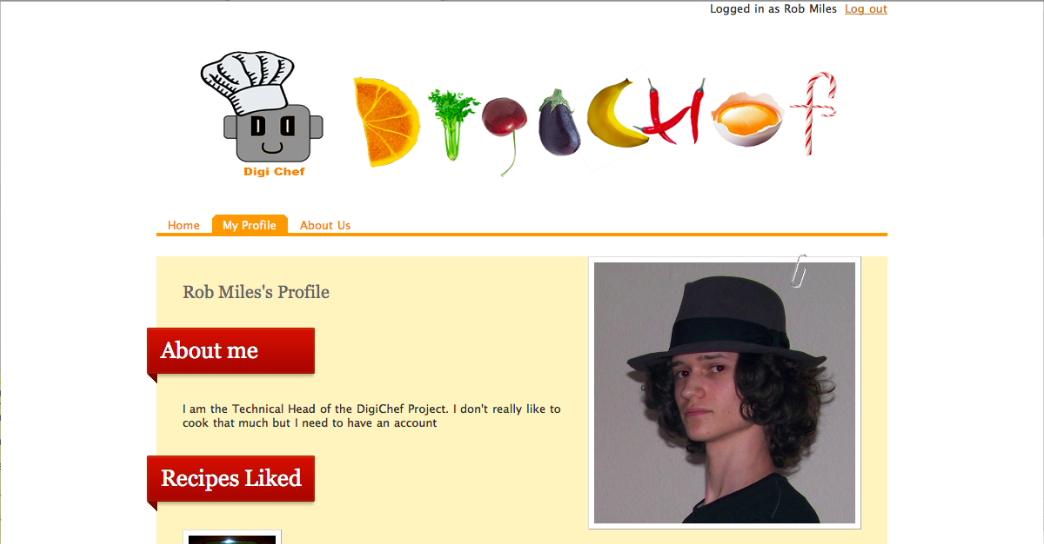
\includegraphics[width=1\textwidth]{result_profile}[H]
\caption{Profile Page}
\label{fig:result_profile}
\end{figure}

Fig~\ref{fig:result_profile} displays how the user profile page looks like. It lists a simple description of the user, shows the users profile picture, the recipes which the user liked, and also the recipes which are recommended to the user. Additionally, from this page, the user could choose to edit his profile as shown in Fig~\ref{fig:editprofile} or even add a new recipe as shown in Fig~\ref{fig:addrecipe}.


\begin{figure}[H]
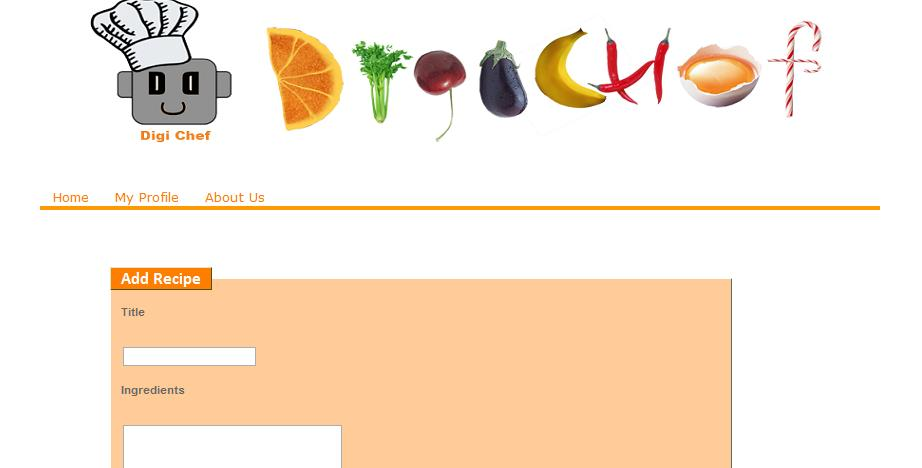
\includegraphics[width=1\textwidth]{addrecipe}[H]
\caption{Submitting you own recipe}
\label{fig:addrecipe}
\end{figure}


\begin{figure}[H]
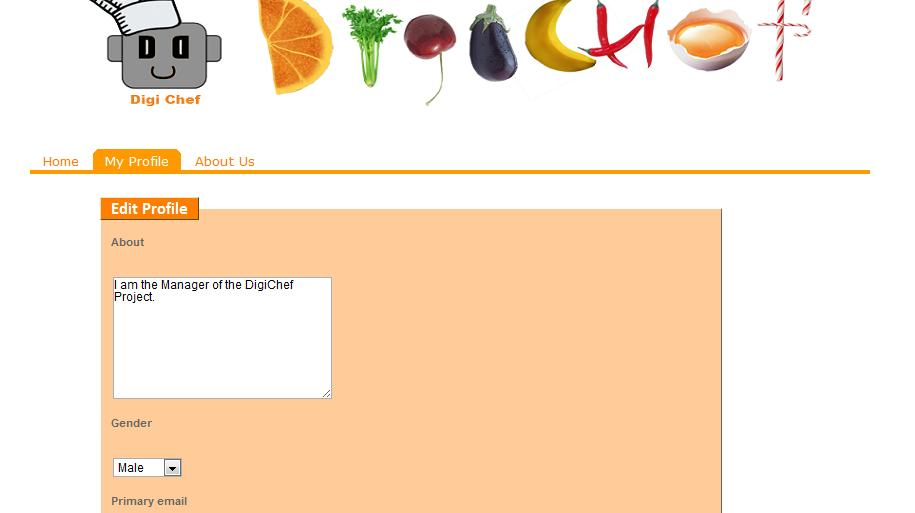
\includegraphics[width=1\textwidth]{editprofile}[H]
\caption{Editing your profile page}
\label{fig:editprofile}
\end{figure}



\begin{figure}[H]
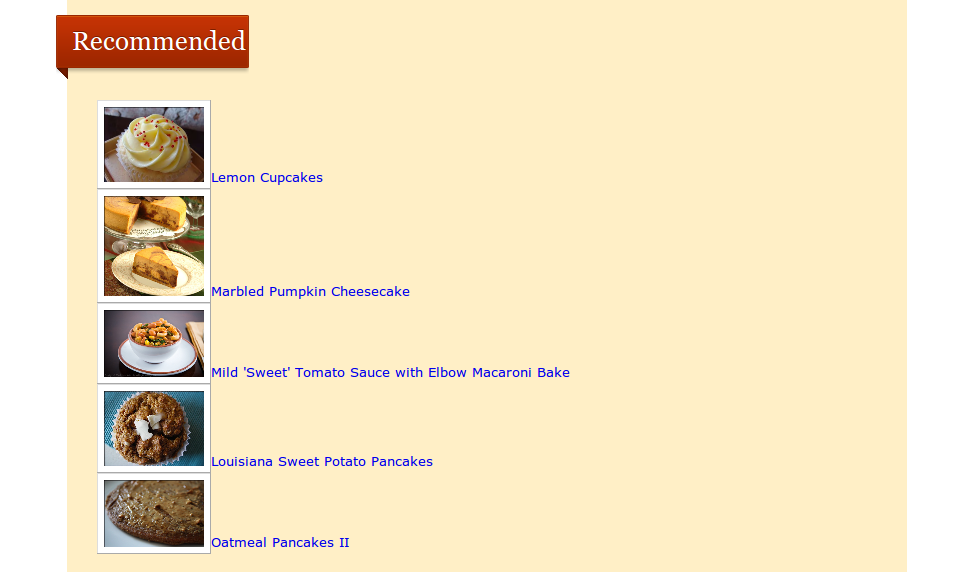
\includegraphics[width=1\textwidth]{recommendations}[H]
\caption{Profile Page}
\label{fig:recommendations}
\end{figure}

Fig~\ref{fig:recommendations} shows the outcome of the recommendation. The "Recommend" section shows a list of recipes automatically generated by the system based on the collaborative filtering algorithm. This list is based on users' vote history and the other users' history if they have same interest with the user.
